\documentclass[12pt]{beamer}

% INCLUDE GRAPHICS
\usepackage{graphicx}

% TABLES
\newcommand{\ra}[1]{\renewcommand{\arraystretch}{#1}} % spaces in tables
\usepackage{booktabs}   % Allows the use of \toprule, \midrule and \bottomrule in tables for horizontal lines

% FONTS
% PdfLatex
% \usepackage[T1]{fontenc}
% \usepackage{pgf}
% \logo{\pgfputat{\pgfxy(-1,-0.435)}{\pgfbox[center,base]{
\includegraphics[width=1.2cm,natwidth=610,natheight=642]{KUNATLogo.pdf}}}}

% FONTS
% xelatex
\usepackage{fontspec}
% \fontspec[Path=../fonts/,]{
%     UprightFont = *-regular,
%     ItalicFont = *-italic,
%     Boldfont = *-bold
% }

% NOTE
% Add fonts to ~/.fonts for this to work
% \setsansfont{TeX Gyre Heros}
% \setsansfont{TeX Gyre Heros Cn}
% \setsansfont{Liberation Sans}
\setsansfont{Muli}
% \setsansfont{Helvetica Neue}

% Monospaces font
\setmonofont{Monaco}

% Use serif for Math environments
\usefonttheme[onlymath]{serif}

% TODO Use mono fonts

% CODE
\usepackage{listings} % Code block (source code) \begin{lstlisting}
\lstset{
    language=Python,                        % Code langugage
    commentstyle=\color{gray},              % Comments font
    basicstyle=\scriptsize\ttfamily,             % Code font, Examples: \footnotesize, \ttfamily
    keywordstyle=\bfseries\color{blue},
    stringstyle=\color{orange},
    numbers=left,                           % Line nums position
    numberstyle=\tiny,                      % Line-numbers fonts
    stepnumber=1,                           % Step between two line-numbers
    numbersep=5pt,                          % How far are line-numbers from code
    numbers=none,
    frame=lines,                             % A frame around the code
    rulecolor=\color{gray},
    tabsize=4,                              % Default tab size
    captionpos=b,                           % Caption-position = bottom
    breaklines=true,                        % Automatic line breaking?
    breakatwhitespace=false,                % Automatic breaks only at whitespace?
    showspaces=false,                       % Dont make spaces visible
    showstringspaces=false,                 % Dont make spaces visible in strings
    showtabs=false,                         % Dont make tabls visible
    belowskip=5pt,
    morekeywords={range, xrange},
    backgroundcolor=\color{white}
    % emph={[2]root,base}
    % morekeywords={one,two,three,four,five,six,seven,eight,
}

\newcommand{\code}[1]{{\small\ttfamily #1}} % \code{inline code}

%
% COLORS
%
\definecolor{kugreen}{RGB}{50,93,61}

\definecolor{orange}{RGB}{255,127,0}
\definecolor{green}{RGB}{0,153,51}
\definecolor{blue}{RGB}{3,115,187}
\definecolor{red}{RGB}{221,17,68}
\definecolor{gray}{RGB}{55,55,55}
\definecolor{black}{RGB}{0,0,0}

\definecolor{offwhite}{RGB}{249,242,215}
\definecolor{foreground}{RGB}{23,23,23}
\definecolor{background}{RGB}{255,255,255}
\definecolor{subtitle}{RGB}{102,255,204}
\definecolor{hilight}{RGB}{102,255,204}
\definecolor{vhilight}{RGB}{255,111,207}
\definecolor{lolight}{RGB}{155,155,155}


%
% BEAMER STYLE COLORS
%
\setbeamercolor{titlelike}{fg=black}
\setbeamercolor{subtitle}{fg=blue}
\setbeamercolor{institute}{fg=gray}
\setbeamercolor{normal text}{fg=foreground,bg=background}
\setbeamercolor{item}{fg=foreground} % color of bullets
\setbeamercolor{subitem}{fg=gray}
\setbeamercolor{itemize/enumerate subbody}{fg=gray}

\setbeamerfont{itemize/enumerate subbody}{size=\footnotesize}
\setbeamerfont{itemize/enumerate subitem}{size=\footnotesize}

\setbeamerfont{footnote}{size=\tiny}

\setbeamersize{text margin left=10pt}
\setbeamersize{text margin right=10pt}
\setbeamersize{sidebar width right=0pt}
\setbeamersize{sidebar width left=0pt}

%
% REMOVES THE NAVIGATION BAR
%
\beamertemplatenavigationsymbolsempty


% BEAMER TEMPLATES


%
% BEAMER BACKGROUND
%
\usebackgroundtemplate{

    \rule{0pt}{0.97\paperheight}%
    \hspace*{1.15\paperwidth}%
    \makebox[0pt][r]{%
        
\includegraphics[width=100pt,natwidth=610,natheight=642]{KUNATLogo.pdf}
    }

}


%
% BEAMER HEADLINE
%
\setbeamertemplate{headline}{}


%
% BEAMER TITLE
%
\setbeamertemplate{frametitle}
{
    \begin{centering}
    \insertframetitle\par
    \end{centering}
}


%
% BEAMER FOOTER
%
\setbeamertemplate{footline}[text line]
{%
    \vbox{%
        \insertvrule{0.5pt}{kugreen}

        \vspace{2pt}

        \strut{
        % \rmfamily\itshape
        \expandafter\insertshorttitle
        \expandafter\insertauthor
        \insertshortinstitute
        }
        \hfill\strut{
        }
        \hfill\strut{
            \insertframenumber\,/\,\inserttotalframenumber
        }

        \vspace{1pt}
    }
}


%
% TITLE PAGE
%
% \setbeamertemplate{title page}
% {
%     % Remove beamer background
%     \setbeamertemplate{background}{}
% 
%     \begin{beamercolorbox}[center]{beamer color}
% 
%         {
%             \huge
%             \color{kugreen}
%             \inserttitle
%         }
%         \bigskip
%         \bigskip
% 
%         % 
\includegraphics[width=2cm]{KUNATLogo}
% 
%         \bigskip
%         {
%             \bf
%             \rmfamily
%             {\large \insertauthor}
%         }
% 
%         \smallskip
%         {
%             \rmfamily
%             \footnotesize
%             \insertinstitute
%         }
% 
%         {
%             \rmfamily
%             \footnotesize
%             \insertdate
%         }
% 
%     \end{beamercolorbox}
% 
%     % Do not count the title page
%     \addtocounter{framenumber}{-1}
% }


% PSTRICKS
\usepackage{pstricks,pst-node,pst-tree} % includes graph additions
% \usepackage{pst-pdf}	% Compiles the pictures
\usepackage{pst-node}
\usepackage{pst-plot}
\usepackage{pst-3dplot}
\usepackage{pstricks-add}


% TITLE AND OTHER STUFF GOES HERE
\title[University of Copenhagen]{Molecular Statistics, Exam Projects}
\author{
    % Jimmy C. Kromann - jimmy@charnley.dk
    % \newline
    % Lars A. Bratholm - larsbratholm@gmail.com\\
}

\date{}

\begin{document}

\frame[plain]{\titlepage}


% ***************************************************
% BEGIN FRAMES
% ***************************************************

\frame
{
    \frametitle{Projects}

    \begin{enumerate}
      \item Diffusion Coefficient of the Lennard-Jones Fluid
      \item Genetic Algorithm
      \item Ising Spin-Lattice
    \end{enumerate}
}

\frame
{
    \frametitle{Project 1: Diffusion Coefficient}
    \centering

    Self-diffusion in Lennard-Jones Fluid.

    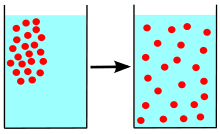
\includegraphics[width=0.2\textwidth]{images/diffusion_illustration.png}

    % \begin{columns}[c]
    %   \column{0.5\textwidth}
    %   \centering
    %
    %     Mean-Square Displacement
    %
    %     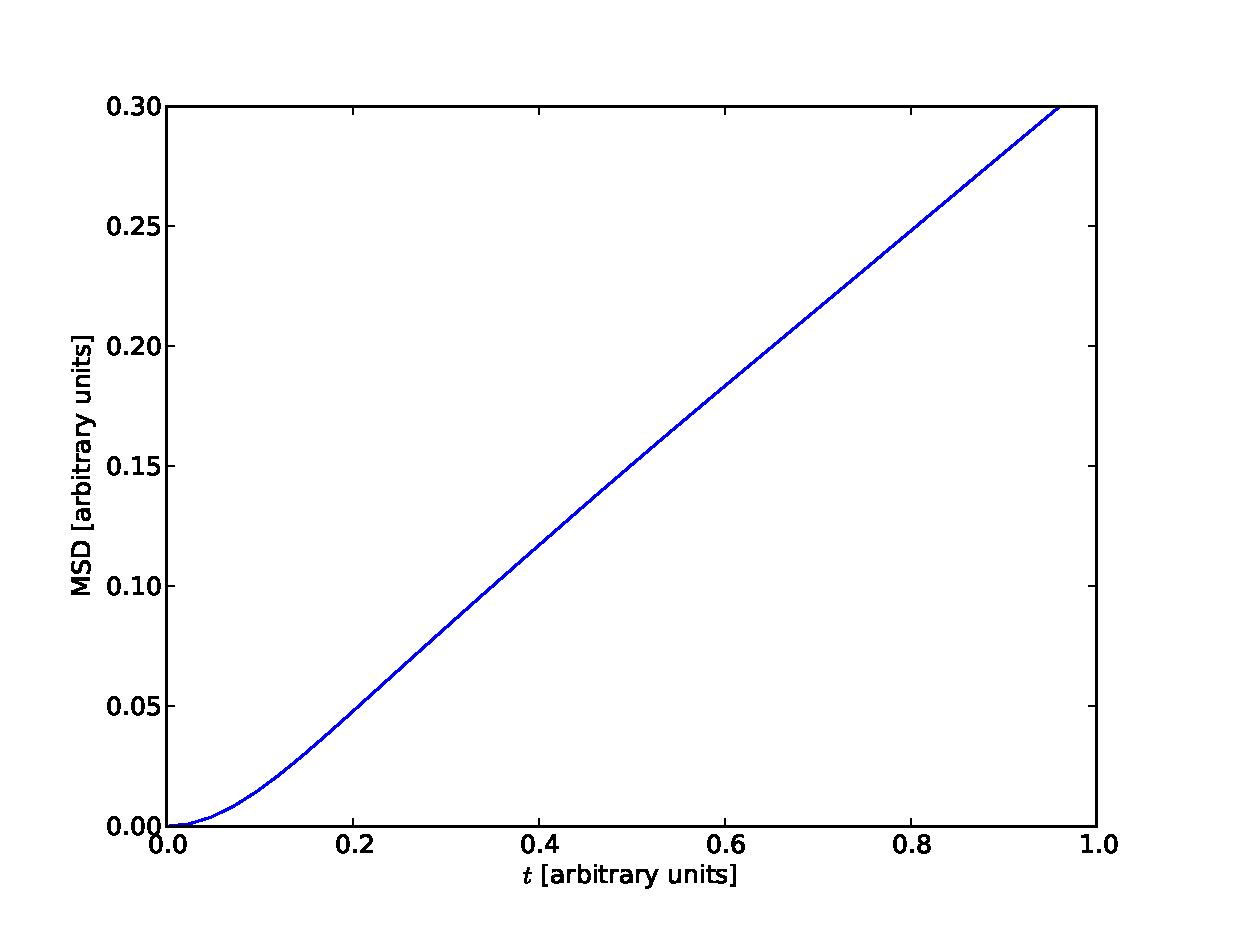
\includegraphics[width=0.8\textwidth]{images/diffusion_msd.eps}
    %
    %   \column{0.5\textwidth}
    %   \centering
    %
    %     Velocity Auto-Correlation Function
    %
    %     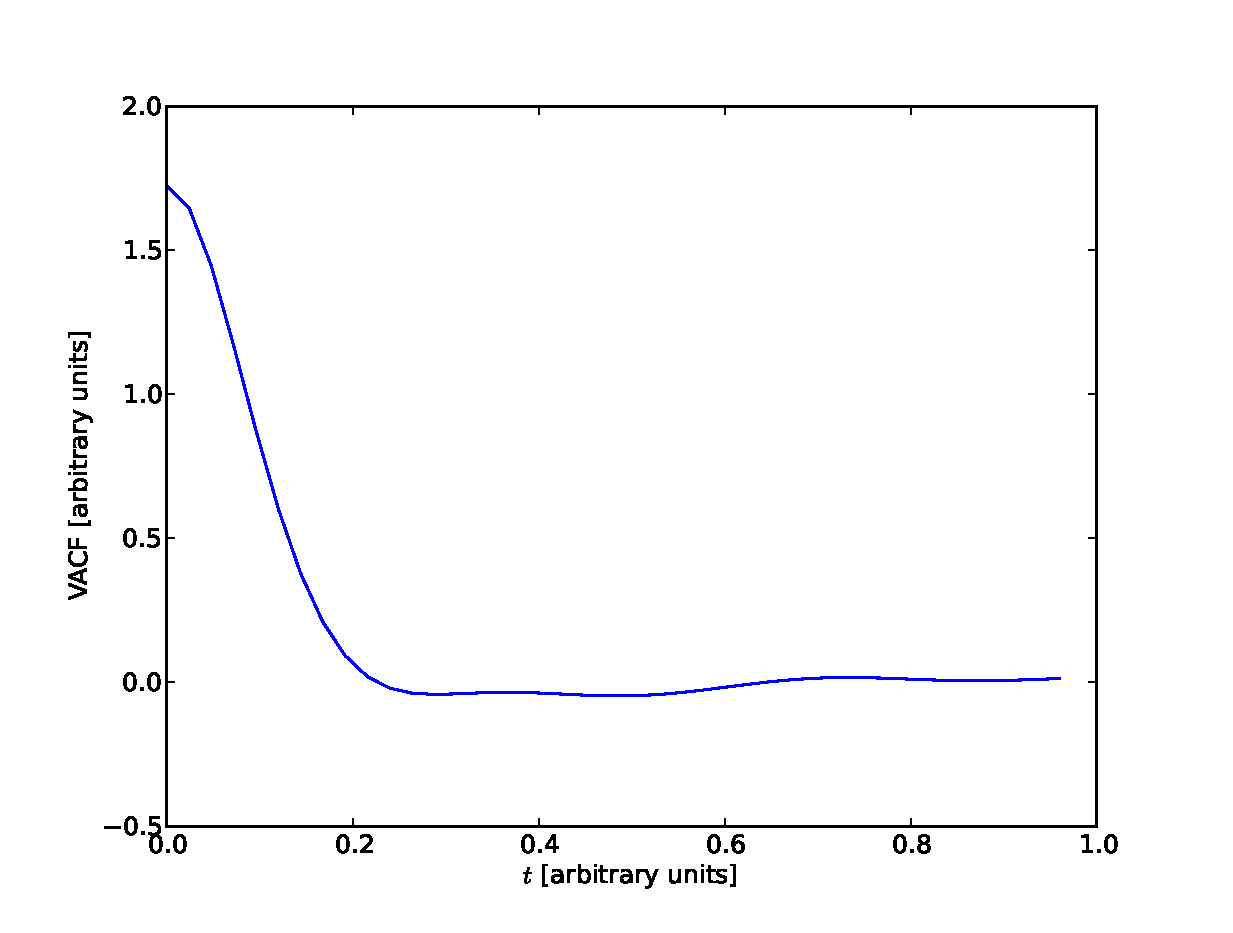
\includegraphics[width=0.8\textwidth]{images/diffusion_vacf.eps}
    %
    % \end{columns}

    \begin{align*}
        D \ \ = \ \ \lim_{t\rightarrow \infty} \frac{\mathrm{MSD}(t)}{4t}
          \ \ = \ \ \frac{1}{2} \int_0^\infty \mathrm{VACF}(t) \ \ dt
    \end{align*}

}


\frame
{
  \frametitle{Project 1: Diffusion Coefficient}
  {\bf Project description:}

  \smallskip

  \begin{itemize}
    \item Simulate diffusion under different simulation conditions
            (pressure, temperature, etc.) using MD in Python.
    \vspace{0.2in}
    \item Calculate MSD and VACF.
    \vspace{0.2in}
    \item Calculate diffusion coefficients.
  \end{itemize}

}


\frame
{
    \frametitle{Project 2: Genetic Algorithm}

    \centering
    {\bf Genetic Algorithm}

    \begin{center}
        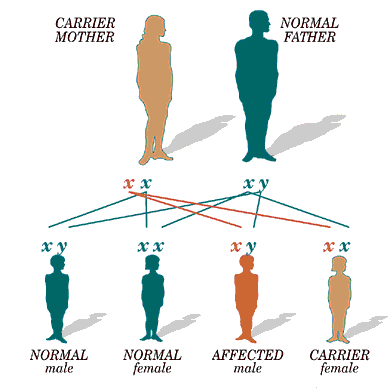
\includegraphics[width=0.5\textwidth]{images/genetics_family.png}
    \end{center}
}


\frame
{
    \frametitle{Project 2: Genetic Algorithm}

    \begin{center}
    Energy as a function of dihedral angles
    \end{center}

    \begin{columns}[c]
      \column{0.5\textwidth}

\begin{figure}
	\psset{xunit=0.8cm,yunit=0.8cm}
    \begin{pspicture}(-2,-3)(4,3)
        \psframe(-2,-3)(4,3)
        \psline{->}(0.0,0.0)(2.0,0.0)
        \rput{60.0}(0.0,0.0)
        {
            \psline{->}(-2.0,0.0)(0.0,0.0)
            \pscircle(-2.0,0.0){0.3}
        }
        \rput{60.0}(2.0,0.0)
        {
            \psline{->}(0.0,0.0)(2.0,0.0)
            \pscircle(2.0,0.0){0.3}
        }

        % Circles
        \pscircle(0.0,0.0){0.3}
        \pscircle(2.0,0.0){0.3}
        \rput(3.0,0.0){.}
        \psellipse[linestyle=dashed](3.0,0.0)(0.2,1.7)
        \psellipse[linestyle=dashed](1.0,0.0)(0.15,0.6)
        \psframe*[linecolor=white](0.84,0.1)(1.16,0.7)
        \parabola{->}(0.85,0.0)(1.0,0.6)
        \rput(1.15,0.8){$\omega$}
        \rput(-1.5, -1.4){A}
        \rput(-0.4, 0.4){B}
        \rput(2.0, -0.6){C}
        \rput(2.6, 2.1){D}
    \end{pspicture}
\end{figure}

        \column{0.5\textwidth}

            \centering

            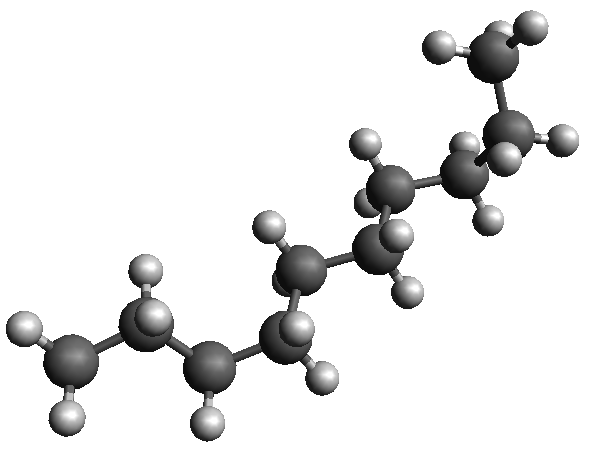
\includegraphics[width=0.8\textwidth]{images/genetics_unsorted.png}


    \end{columns}

}


\frame
{
    \frametitle{Project 2: Genetic Algorithm}

    \begin{columns}[c]
      \column{0.5\textwidth}
      \centering
      Parent

      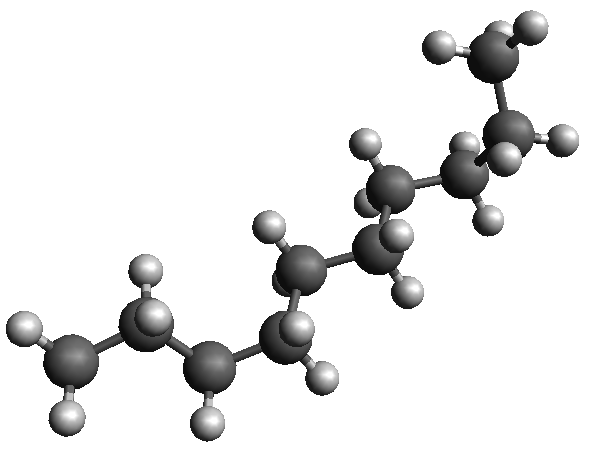
\includegraphics[width=0.4\textwidth]{images/genetics_unsorted.png}

      High energy

      \column{0.5\textwidth}
      \centering
      Child

      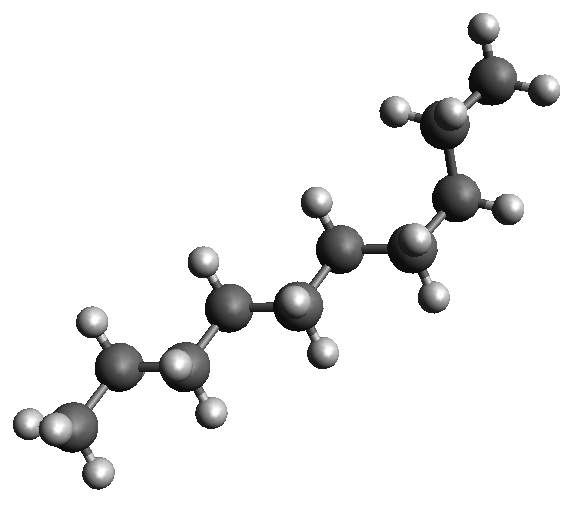
\includegraphics[width=0.4\textwidth]{images/genetics_sorted.png}

      Low energy

    \end{columns}

    \qquad
    \newline
    \qquad

    {\bf Project description:}
    \begin{itemize}

        \item Implement the genetic algorithm in Python.

        \smallskip

        \item Use a force field to calculate molecular energies.

        \smallskip

        \item Use the genetic algorithm to energy minimize alkane 
                molecular structures.

    \end{itemize}
}

\frame
{
    \frametitle{Project 3: 2D Ising Model}

    \begin{center}
        Representation of 2D magnetic solid
    \end{center}

    \bigskip

    \begin{columns}[c]

        \column{0.5\textwidth}

            \centering

            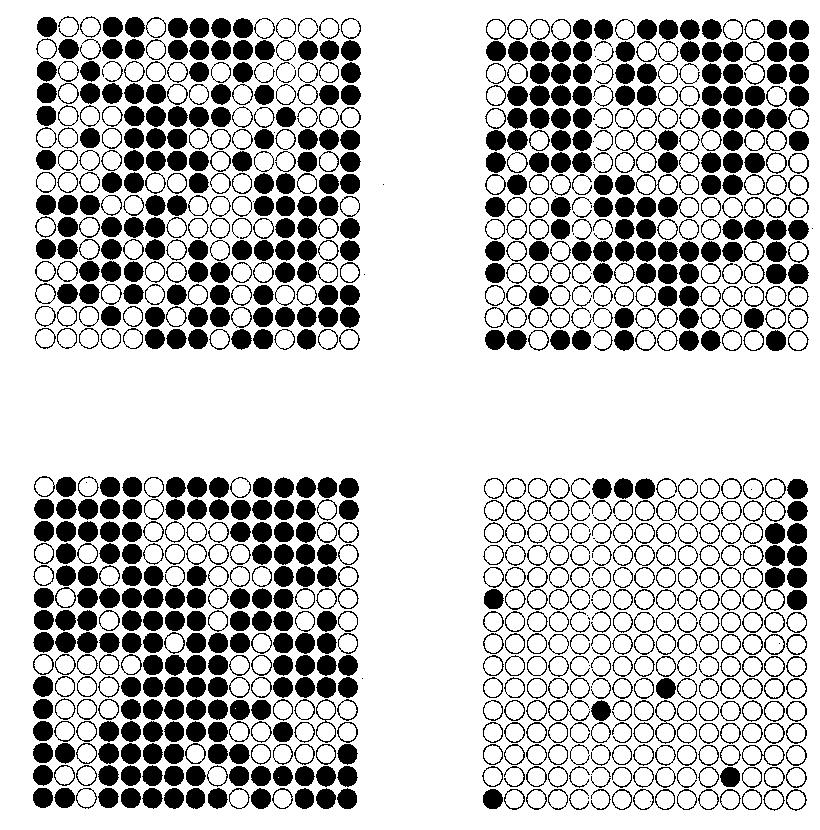
\includegraphics[width=0.7\textwidth]{images/temperatures.png}


        \column{0.5\textwidth}

            \centering

            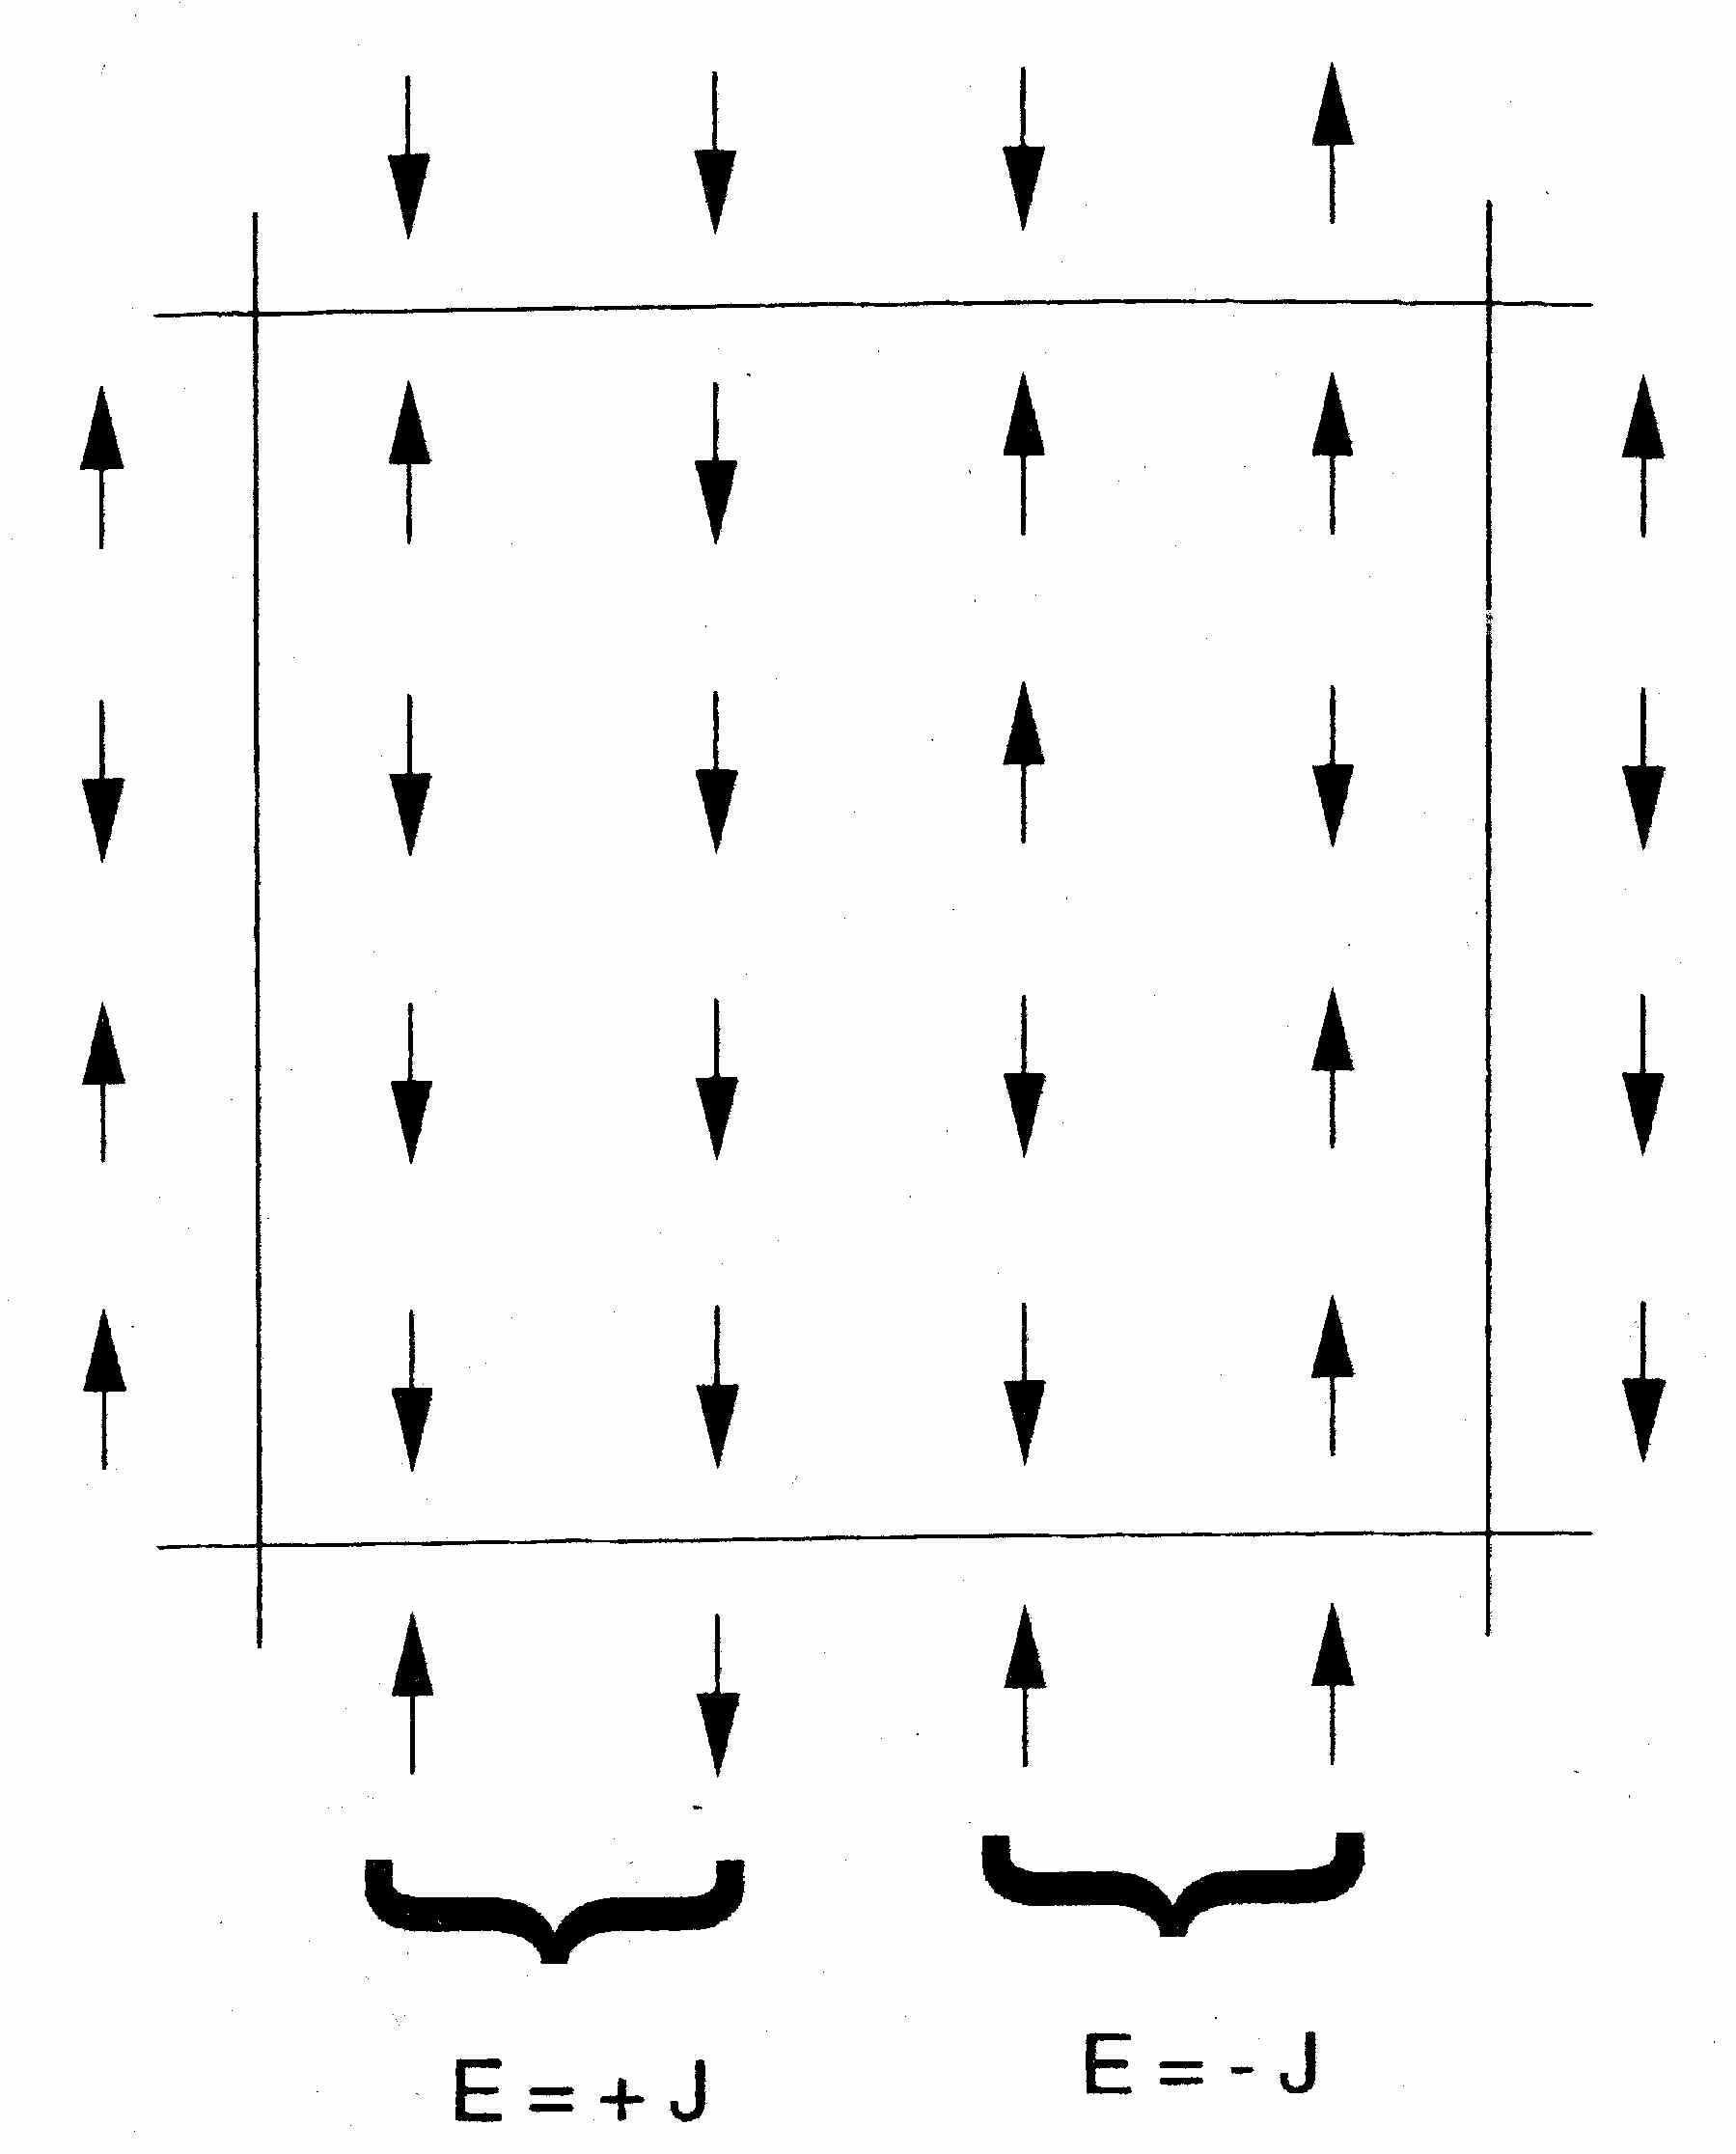
\includegraphics[width=0.7\linewidth]{images/lattice.png}

    \end{columns}

}


\frame
{
    \frametitle{Project 3: 2D Ising Model}

    \textbf{Project description:}

    \bigskip

    \begin{itemize}

        \item Simulate the 2D Ising spin lattice.

        \bigskip

        \item Implement the Monte Carlo Metropolis-Hastings algorithm.

        \bigskip

        \item Calculate properties such as heat capacity, magnetization, and magnetic susceptibility.

    \end{itemize}

}


\frame
{

    \frametitle{Project description}

    \textbf{General:}

    \begin{itemize}

        \item Programming is done in small groups

        \item The reports are individual.

        \item The language is Danish or English.

    \end{itemize}

    \bigskip


    \textbf{\code{if stuck}:}

    \begin{enumerate}

        \item Collaborate with other groups

        \item Write an email and make an appointment to meet with a TA

    \end{enumerate}

}


% ***************************************************
% END FRAMES
% ***************************************************

\end{document}

